

\documentclass[10pt,a5paper,twoside]{article}

% ==========================================
% 1. MATHEMATICS AND LANGUAGE
% ==========================================

\usepackage{amsfonts,amssymb,amsmath}

\usepackage[
banglamainfont=Kalpurush,
banglattfont=Siyam Rupali
]{latexbanglapatch}

\usepackage{fontspec}
\usepackage{polyglossia}



% ==========================================
% 2. PACKAGES
% ==========================================

\usepackage[shortlabels]{enumitem}

\usepackage[
paperwidth=148mm,
paperheight=210mm,
top=18mm,
bottom=17mm,
inner=17mm,
outer=14mm,
headheight=30pt,
headsep=7mm,
footskip=8mm
]{geometry}

\usepackage{graphicx}
\usepackage{fancyhdr}
\usepackage{float}
\usepackage{caption}
\usepackage[super]{nth}
\usepackage{xcolor}
\usepackage{etoolbox}
\usepackage{mathabx}
\usepackage{ifsym}
\usepackage{siunitx}
\usepackage{wrapfig}
\usepackage{multicol}
\usepackage{tcolorbox}
\usepackage{bm}
\usepackage{lastpage}
\usepackage{tikz}
\usepackage{adjustbox}
\usepackage{tocloft}

\tcbuselibrary{hooks,breakable,skins}
\usetikzlibrary{calc}

% Compact table of contents for A5
\renewcommand{\cfttoctitlefont}{\Large\bfseries}
\renewcommand{\cftaftertoctitle}{\par\vspace{0.4em}}
\renewcommand{\cftsecfont}{\small\normalfont}
\renewcommand{\cftsecpagefont}{\small\normalfont}
\renewcommand{\cftsubsecfont}{\footnotesize\normalfont}
\renewcommand{\cftsubsecpagefont}{\footnotesize\normalfont}
\setlength{\cftbeforesecskip}{3pt}
\setlength{\cftbeforesubsecskip}{1pt}
\setlength{\cftsecnumwidth}{2.0em}

% ==========================================
% GLOBAL LIST SPACING
% ==========================================

\setlist{
	itemsep=0em
}

\newcommand{\prr}{\\[-0.9\baselineskip]}
%\usepackage[hidelinks]{hyperref}

% ==========================================
% 3. BOOKLET INFORMATION
% ==========================================

\newcommand{\BookTitle}{BDOAA Problem Booklet}
\newcommand{\BookYears}{2018--2026}

\newcommand{\OlympiadName}{%
	Bangladesh Olympiad on Astronomy and Astrophysics%
}

\newcommand{\PublisherName}{%
	Bangladesh Olympiad on Astronomy and Astrophysics Committee%
}

\newcommand{\PublicationYear}{2026}
\newcommand{\EditionName}{First Edition}

% ==========================================
% 4. GRAPHICS
% ==========================================

\graphicspath{{./images/}}

% Main organizational logo
\newcommand{\BDOAALogo}[1]{%
	
\includegraphics[width=#1]{bdoaa_logo.png}%
}

% ==========================================
% 5. COVER COLOURS
% ==========================================

\definecolor{covermain}{HTML}{F15B53}
\definecolor{coveraccent}{HTML}{FCC860}

% Darker version of the main colour
\colorlet{coverdark}{covermain!55!black}

% Horizontal title band
\definecolor{coverband}{HTML}{1E1B1B}

% ==========================================
% 6. EDITABLE COVER TEXT
% ==========================================

\newcommand{\CoverBookletText}{Problem Booklet}
\newcommand{\CoverYearText}{2018--2026}

\newcommand{\CoverMainTitle}{%
	Bangladesh Olympiad on Astronomy and Astrophysics%
}

\newcommand{\CoverOrgText}{%
	Bangladesh Olympiad\\
	on Astronomy and\\
	Astrophysics Committee%
}

\newcommand{\CoverPlaceYear}{Bangladesh, 2026}

% ==========================================
% 7. GENERAL TYPOGRAPHY
% ==========================================

\setlength{\parindent}{0pt}
\setlength{\parskip}{0.35em}

\setcounter{secnumdepth}{2}
\setcounter{tocdepth}{2}

% ==========================================
% 8. HEADER AND FOOTER
% ==========================================

% Automatically use the current section
% as the chapter title in the running header.
%
% Since the document uses the article class,
% sections function as chapters.

\renewcommand{\sectionmark}[1]{%
	\markboth{#1}{}%
}

\fancypagestyle{bdoaa}{%
	
	% Clear all header and footer fields
	\fancyhf{}
	
	% --------------------------------------
	% EVEN PAGES — LEFT-HAND PAGES
	% Page number | Chapter name
	% --------------------------------------
	
	\fancyhead[LE]{%
		\small
		\normalfont\bfseries\thepage
		\hspace{1.5em}%
		\normalfont\itshape\nouppercase{\leftmark}%
	}
	
	% --------------------------------------
	% ODD PAGES — RIGHT-HAND PAGES
	% Chapter name | Page number
	% --------------------------------------
	
	\fancyhead[RO]{%
		\small
		\normalfont\itshape\nouppercase{\leftmark}%
		\hspace{1.5em}%
		\normalfont\bfseries\thepage
	}
	
	% --------------------------------------
	% NO HEADER OR FOOTER RULES
	% --------------------------------------
	
	\renewcommand{\headrulewidth}{0pt}
	\renewcommand{\footrulewidth}{0pt}
}







% ==========================================
% 9. PROBLEM HEADING AND NUMBERING
% ==========================================

% Problem counter:
% 1.1, 1.2, ..., 2.1, 2.2, ...
\newcounter{problem}[section]

\renewcommand{\theproblem}{%
	\thesection.\arabic{problem}%
}

% Problem source colour
\definecolor{problemsource}{HTML}{777777}

\newcommand{\pr}[3]{%
	\par\addvspace{1.2em}%
	\refstepcounter{problem}%
	\phantomsection%
	\addcontentsline{toc}{subsection}{%
		\protect\numberline{}%
		\theproblem
	}%
	\noindent
	\begin{minipage}[c]{0.65\linewidth}
		\raggedright
		\bfseries
		\theproblem\enspace #1
	\end{minipage}%
	\hfill
	\begin{minipage}[c]{0.34\linewidth}
		\raggedleft
		\normalfont\small
		\color{problemsource}%
		\textsc{BDOAA/#2/#3}%
	\end{minipage}%
	\par\nobreak
	\vspace{-1.3em}%
	\noindent\rule{\linewidth}{0.4pt}%
	\par\nobreak
	\vspace{0.5em}%
}

% ==========================================
% 10. PROBLEM MARKS
% ==========================================

% Usage: \m{4} produces (4pt)
% Right-aligned within the text area.

\newcommand{\m}[1]{%
	\unskip\nobreak\hfill
	\mbox{\normalfont(#1pt)}%
}


% ==========================================
% DOCUMENT BEGINS
% ==========================================

\begin{document}
	
	% Suppress folios on all front-matter pages.
	% Do not create PDF page anchors until the main numbered text.
	\pagenumbering{gobble}
	\pagestyle{empty}
	\hypersetup{pageanchor=false}
	
	% ==========================================
	% PAGE 1 — TIKZ FRONT COVER
	% ==========================================
	
	\begin{titlepage}
		\thispagestyle{empty}
		
		\begin{tikzpicture}[remember picture,overlay]
			
			% ------------------------------------------
			% FULL-PAGE BACKGROUND
			% ------------------------------------------
			
			\fill[covermain]
			(current page.south west)
			rectangle
			(current page.north east);
			
			% ------------------------------------------
			% RIGHT DARK PANEL
			% ------------------------------------------
			
			\fill[coverdark]
			($(current page.north west)
			+(0.64\paperwidth,0)$)
			rectangle
			(current page.south east);
			
			% ------------------------------------------
			% VERTICAL ACCENT STRIP
			% ------------------------------------------
			
			\fill[coveraccent]
			($(current page.north west)
			+(0.615\paperwidth,0)$)
			rectangle
			($(current page.south west)
			+(0.64\paperwidth,0)$);
			
			% ------------------------------------------
			% UPPER-RIGHT BOOKLET LABEL
			% ------------------------------------------
			
			\node[
			anchor=north west,
			text=white,
			align=left,
			inner sep=0pt,
			text width=0.30\paperwidth
			] at
			($(current page.north west)
			+(0.665\paperwidth,-0.165\paperheight)$)
			{%
				\sffamily\bfseries
				\fontsize{12}{14}\selectfont
				\CoverBookletText\\[2pt]
				\CoverYearText
			};
			
			% ------------------------------------------
			% HORIZONTAL TITLE BAND
			% ------------------------------------------
			
			\fill[coverband]
			($(current page.north west)
			+(0,-0.265\paperheight)$)
			rectangle
			($(current page.north west)
			+(0.915\paperwidth,-0.327\paperheight)$);
			
			% Main title
			\node[
			anchor=center,
			text=white,
			inner sep=0pt
			] at
			($(current page.north west)
			+(0.4575\paperwidth,-0.296\paperheight)$)
			{%
				\adjustbox{max width=0.85\paperwidth}{%
					\sffamily\bfseries
					\fontsize{17}{20}\selectfont
					\CoverMainTitle
				}%
			};
			
			% ------------------------------------------
			% CENTRAL ASTRONOMICAL PHOTOGRAPH
			% ------------------------------------------
			
			% Photograph area:
			% Width  = 78% of page width
			% Height = 36.5% of page height
			%
			% Image aspect ratio is preserved.
			% Excess image content is cropped.
			
			
			\begin{scope}
				
				\clip
				($(current page.north west)
				+(0.18\paperwidth,-0.365\paperheight)$)
				rectangle
				($(current page.north west)
				+(0.96\paperwidth,-0.730\paperheight)$);
				
				\node[
				anchor=center,
				inner sep=0pt
				] at
				($(current page.north west)
				+(0.57\paperwidth,-0.5475\paperheight)$)
				{%
					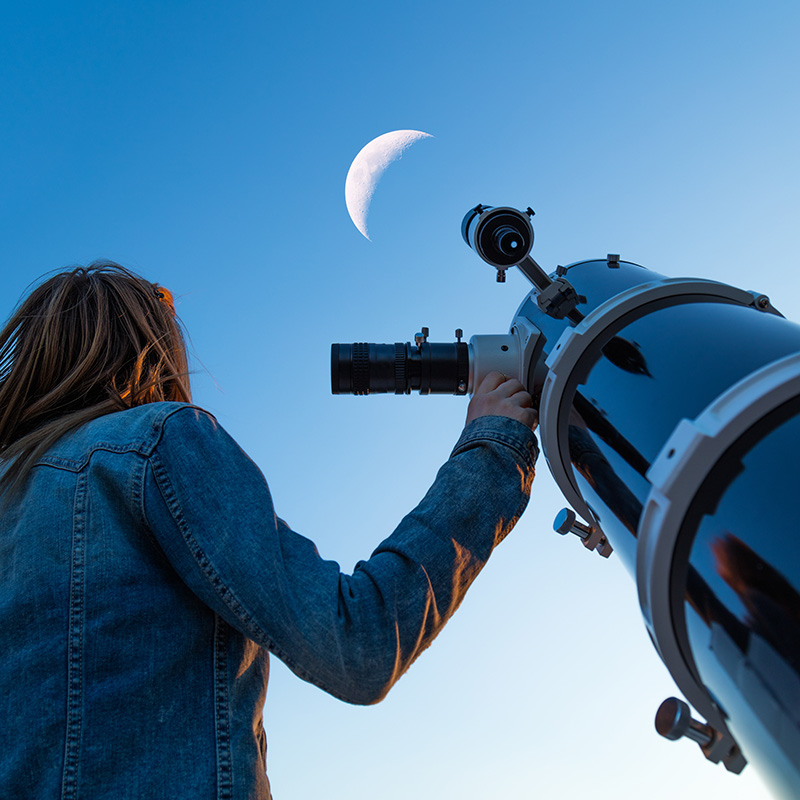
\includegraphics[
					width=0.78\paperwidth
					]{cover00}
				};
				
			\end{scope}
			
			
			% ------------------------------------------
			% LOWER-RIGHT ORGANIZER INFORMATION
			% ------------------------------------------
			
			\node[
			anchor=north west,
			text=white,
			align=left,
			inner sep=0pt,
			text width=0.30\paperwidth
			] at
			($(current page.north west)
			+(0.665\paperwidth,-0.805\paperheight)$)
			{%
				\sffamily\bfseries
				\fontsize{9.5}{12}\selectfont
				
				\CoverOrgText
				
				\par\vspace{7mm}
				
				\CoverPlaceYear
			};
			
		\end{tikzpicture}
		
		\null
	\end{titlepage}
	
	% ==========================================
	% PAGE 2 — INNER TITLE PAGE
	% ==========================================
	
	\thispagestyle{empty}
	
	\begin{center}
		
		\vspace*{2.3cm}
		
		{\fontsize{22}{22}\selectfont
			\textsc{Bangladesh Olympiad\\
				on Astronomy and Astrophysics}
			\par}
		
		\vspace{0.75cm}
		
		{\fontsize{17}{22}\selectfont
			Problem Booklet
			\par}
		
		\vspace{0.1cm}
		
		{\fontsize{15}{19}\selectfont
			2018--2026
			\par}
		
		\vspace{1.2cm}
		
		{\normalsize
			Compiled and edited by
			\par}
		
		\vspace{0.1cm}
		
		{\large
			BDOAA Academic Team
			\par}
		
		
		\vfill
		
		% BDOAA logo near the bottom
		
		\BDOAALogo{0.36\textwidth}
		
		\vspace{1cm}
		
	\end{center}
	
	\clearpage
	
	% ==========================================
	% PAGE 3 — PUBLICATION AND CREDITS
	% ==========================================
	
	\thispagestyle{empty}
	
	
	\begin{flushleft}
		
		\small
		
		\textbf{BDOAA Problem Booklet 2018--2026}
		
		\vspace{0.35cm}
		
		\textbf{Compilation and editing}\\
		Fahim Rajit Hossain Shwadhin, Tasdik Ahmed, Sheikh Alvi\\
		Names to be Added
		
		\vspace{0.35cm}
		
		\textbf{Published by}\\
		Bangladesh Olympiad on Astronomy
		and Astrophysics
		
		\vspace{0.35cm}
		
		\textbf{Edition}\\
		First Edition, 2026
		
		\vspace{0.35cm}
		
		\textbf{Typesetting}\\
		\LaTeX
		
		\vspace{0.35cm}
		
		\textbf{Copyright and licensing: BDOAA}
		
		\vspace{0.35cm}
		
		\textbf{Repository}
		
		{\footnotesize
			\url{https://github.com/Astronomy-Olympiad-BDOAA/BDOAA-Problem-Booklet}
			\par}
		
		\vspace{0.35cm}
		
		This publication is not for sale.
		
	\end{flushleft}
	
	\clearpage



% ==========================================
% FRONT MATTER — NO PAGE NUMBERING
% ==========================================

\clearpage
\pagestyle{empty}
\pagenumbering{gobble}

% ==========================================
% TABLE OF CONTENTS
% ==========================================

\tableofcontents
\clearpage

% ==========================================
% INTRODUCTION
% ==========================================

% Start normal page numbering
\pagenumbering{arabic}

% Suppress running header on this page
\thispagestyle{empty}

% Create a unique hyperlink destination
\phantomsection
\addcontentsline{toc}{section}{Introduction}

% Standalone heading
\begin{center}
	\vspace*{1cm}
	{\Large\bfseries Introduction\par}
\end{center}

\vspace{0.8cm}

International science olympiads are competitions where school students from many countries solve demanding problems that reward understanding over memorisation. The International Olympiad on Astronomy and Astrophysics (IOAA) has been held every year since 2007 and is the most prestigious international competition in astronomy and astrophysics for secondary school students. Each country sends up to five students and two team leaders. The students compete individually in theory, data analysis and night sky observation rounds, which carry 50%, 25% and 25% of the total score.

The Bangladesh Olympiad on Astronomy and Astrophysics (BDOAA) is a non-profit organisation that runs the regional and national olympiads, hosts the national astronomy camp and sends a team to the IOAA. On 8 February 2018, with the approval of the IOAA, BDOAA was recognised as the national body for selecting the Bangladesh team, and it has sent students to the olympiad every year since. It is run largely by former olympiad participants who now train the students who follow them. Since 2020, the national rounds have been supported by the Department of Physical Sciences of Independent University, Bangladesh (IUB), and the olympiad now runs under the Center for Astronomy, Space Science and Astrophysics (CASSA) at IUB. BDOAA also organises workshops, offers career guidance to aspiring astronomers and holds public events to popularise astronomy. \prr

This booklet collects problems from the Regional and National rounds of BDOAA, covering all nine editions from 2018 to 2026. The problems are grouped by topic, such as positional astronomy, celestial mechanics and stellar astrophysics, so that readers can work through one area at a time. Each problem carries a tag showing where it was first set. For example, BDOAA/R/2018 marks a problem from the 2018 Regional round. Most problems are printed in Bengali, and some also include an English version. The marks for each part are shown on the right. We encourage readers to make a serious attempt at every problem, and to check that each answer has sensible units, magnitude and significant figures. \prr 

We hope this booklet will help students preparing for BDOAA and the IOAA, as well as teachers and astronomy clubs looking for good problems to work on with their students.


\vspace{0.5cm}

বাংলাদেশ জ্যোতির্বিজ্ঞান অলিম্পিয়াডের
সমস্যাসংকলনে স্বাগতম।

\clearpage

% ==========================================
% MAIN PROBLEM CHAPTERS
% ==========================================

\pagestyle{bdoaa}

\section{Geometry of Astronomy \& Time }


\pr{Eratosthenes' Experiment}{R}{2019}

আজ থেকে অনেকদিন আগেই Eratosthenes নামে একজন ব্যক্তি পৃথিবীর ব্যাসার্ধ মাপতে সক্ষম হয়েছিলেন কিছু সাধারণ পর্যবেক্ষণের সাহায্যে। তাঁর পরীক্ষার ভিত্তি ছিল যে একটি নির্দিষ্ট দিনে, নির্দিষ্ট জায়গায় পর্যবেক্ষকের ঠিক মাথার উপরে সূর্য থাকলে কোনো উল্লম্ব লাঠির ছায়া থাকবে না। ধরো, এই পরীক্ষাটি আমরা নির্দিষ্ট দিনে না করে দুটি এক মিটার দৈর্ঘ্যের লাঠি দুটি স্থানে উল্লম্বভাবে স্থাপন করলাম। একটি স্থান অন্যটি থেকে $950~\mathrm{km}$ দক্ষিণে। মধ্যাহ্নে (যখন সূর্য local meridian-এ আসে)-এ এই দুটি স্থানে লাঠি দুটির ছায়ার দৈর্ঘ্য পাওয়া গেল যথাক্রমে $0.795$ ও $0.577~\mathrm{m}$।

Long ago, a person named Eratosthenes calculated the radius of the Earth using simple observations. The principle of his experiment was that a vertical stick casts no shadow when the Sun is directly overhead. Suppose we instead place two vertical sticks, each $1~\mathrm{m}$ long, at two locations along the same meridian, with the second location $950~\mathrm{km}$ south of the first. At local noon, the measured shadow lengths at the two locations are $0.795~\mathrm{m}$ and $0.577~\mathrm{m}$, respectively.

\begin{enumerate}[a.]
	
	\item লাঠির ছায়া দেখে পর্যবেক্ষক কীভাবে বুঝবে যে মধ্যাহ্ন হয়েছে? \m{2}
	
	How can an observer determine local noon by monitoring the shadow of a vertical stick?
	
	\item উপরের তথ্যগুলো দিয়ে পৃথিবীর ব্যাসার্ধ নির্ণয় করো। \m{4}
	
	Calculate the radius of the Earth using the given information.
	
	\item নিহাল $5895~\mathrm{m}$ উঁচু একটি পাহাড়ের পাদদেশে সেই লাঠির ছায়ার দৈর্ঘ্য $42~\mathrm{cm}$ পেল। তাহলে পাহাড়টির ছায়ার দৈর্ঘ্য কত হবে? \m{4}
	
	Nihal measured a shadow length of $42~\mathrm{cm}$ for the same $1~\mathrm{m}$ vertical stick at the base of a mountain of height $5895~\mathrm{m}$. Determine the length of the mountain's shadow.
	
\end{enumerate}
\textit{Hint:} The mountain's height is not negligible compared with the Earth's radius for this calculation. Assume that the mountain is sufficiently narrow for its shadow to fall on the Earth's surface.

\clearpage

\pr{To the aid of Arabella}{R}{2022}

On April 16, 1664, one of the members of the Arabella crew found himself on a desert island. Waiting for a hard night, and watching the homemade sun clock, he determined that at noon the length of the shadow from the stick was 5 inches. The shadow was directed to the north. The stick itself was 5 feet long. Help the sailor determine his latitude, knowing that he is in the northern hemisphere. One foot is 12 inches.

১৬ই এপ্রিল, ১৬৬৪ সালে Arabella জাহাজের একজন সদস্য একটি জনমানবহীন দ্বীপে নিজেকে আবিষ্কার করে। কঠিন রাতের অপেক্ষায় এবং কোনোমতে বানানো একটি সূর্যঘড়ি দিয়ে সে বের করল যে মধ্যাহ্নের সময় একটি লাঠির ছায়ার দৈর্ঘ্য ছিল ৫ ইঞ্চি। লাঠিটা ৫ ফুট লম্বা ছিল এবং উত্তরের দিকে তাক করা ছিল। নাবিককে তার অক্ষাংশ জানতে সাহায্য কর।

আমরা জানি এক ফুট ১২ ইঞ্চি।



\clearpage

\pr{Radius of the Earth}{R}{2021}

The scientist named Abu Rayhan Al-Biruni had successfully calculated the radius of the Earth in a different way than that done by the Greek mathematician Eratosthenes. The calculation of the radius of the Earth by this method requires the top of a mountain with height $h$, surrounded by a flat field. The angles of the slopes of the mountain with the ground, $\theta_1$ and $\theta_2$, at points 1 and 2 are measured. The distance $d$ between points 1 and 2 is also measured.

বিজ্ঞানী আবু রায়হান আল-বিরুনী গ্রিক গণিতবিদ ইরাটোস্থেনিস এর উপায় হতে ভিন্ন এক উপায়ে সফলতার সাথে পৃথিবীর ব্যাসার্ধ নির্ণয় করেছিলেন। এই উপায়ে ব্যাসার্ধ নির্ণয়ের জন্য $h$ উচ্চতার একটি পাহাড় আর তার চারপাশে সমতল ভূমি দরকার। দুটি বিন্দু 1 আর 2 হতে পাহাড়ের উন্নতি কোণ যথাক্রমে $\theta_1$ এবং $\theta_2$ নির্ণয় করা হয় এবং 1 আর 2 এর দূরত্ব $d$ নির্ণয় করা হয়।

\begin{enumerate}[a.]
	
	\item Express $h$ in terms of $d$, $\theta_1$, and $\theta_2$. \m{2}
	
	$h$ কে $d$, $\theta_1$ এবং $\theta_2$ এর সাপেক্ষে প্রকাশ করো।
\end{enumerate}
An observer climbed the mountain peak and measured the angle $(\theta=90^\circ-\alpha)$ between the vertical and the tangent from the peak to the Earth's surface. The point where the tangent touches the Earth's surface is the horizon. When the observer is on a higher mountain peak, the horizon will be both farther and at a lower elevation.

একজন পর্যবেক্ষক পাহাড়ের চূড়ায় উঠে উল্লম্ব এবং পাহাড় হতে পৃথিবীর উপর অঙ্কিত স্পর্শকের মধ্যকার কোণ $(\theta=90^\circ-\alpha)$ বের করল। যে বিন্দুতে স্পর্শক পৃথিবীকে স্পর্শ করবে, সে বিন্দু হল দিগন্ত। পর্যবেক্ষক যখন কোনো উঁচু পাহাড়চূড়ায় থাকবে তখন দিগন্ত তার কাছে নিচু এবং বেশি দূরে মনে হবে।

\begin{enumerate}[a.]
	\setcounter{enumi}{1}
	
	\item Sketch the geometry of the mountain, the angle of decline of the horizon $\alpha$, and the radius of the Earth. \m{2}
	
	পাহাড়, পাহাড় হতে দিগন্তের অবনতি কোণ $\alpha$, পৃথিবীর ব্যাসার্ধের ছবি আঁকো।
	
	\item Explain the method of Al-Biruni: how he measured the radius of the Earth by repeating the process yourself. Calculate the height of the mountain $h$ and measure the angle of decline of the horizon $\alpha$. \m{2+2}
	
	আল-বিরুনী পাহাড়ের উচ্চতা $h$ এবং দিগন্তের অবনতি কোণ $\alpha$ নির্ণয় করে যে পদ্ধতিতে পৃথিবীর ব্যাসার্ধ নির্ণয় করেছিলেন, সে পদ্ধতি নিজে করে দেখাও।
	
\end{enumerate}

\pr{Illumination of Moon}{R}{2020}

\begin{wrapfigure}{r}{0.35\linewidth}
	\vspace{-0.8cm}
	\centering
	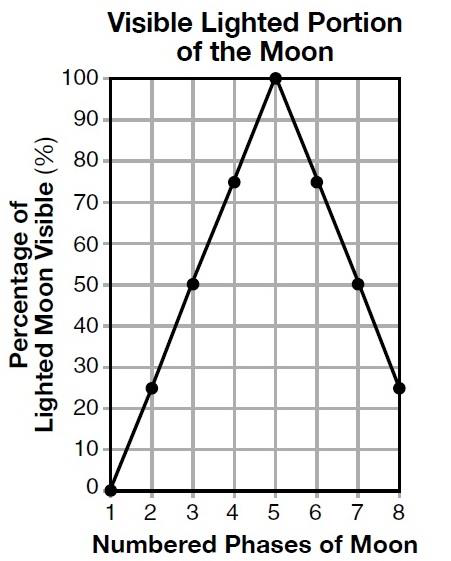
\includegraphics[width=\linewidth]{bdoaa18_r_moonphase}
	\vspace{-2cm}
\end{wrapfigure}



পাশের চিত্রটি ৮টি চন্দ্রকলায় (Lunar Phase) চাঁদের যে পরিমাণ অংশ দেখা যায়, তার শতকরা পরিমাণ নির্দেশ করে।

\begin{enumerate}[a.]
	\item যখন চাঁদ ৪র্থ পর্যায়ে ছিল, তখন চাঁদ-পৃথিবী-সূর্য কী অবস্থানে ছিল, এঁকে দেখাও। \m{3}
	
	\item ধরে নাও, চাঁদের ১ম পর্যায় থেকে ৫ম পর্যায়ে যেতে সময় লাগে ১৪ দিন। তাহলে ১০ দিনে চাঁদের কত শতাংশ আলোকিত অংশ দেখা যাবে? \m{3}
	
	\item ২য় এবং ৭ম পর্যায়ে চাঁদের উজ্জ্বলতার পার্থক্য কত Magnitude? \m{4}
\end{enumerate}


\pr{Golden Gate Bridge!}{R}{2020}

\begin{figure}[H]
	\centering
	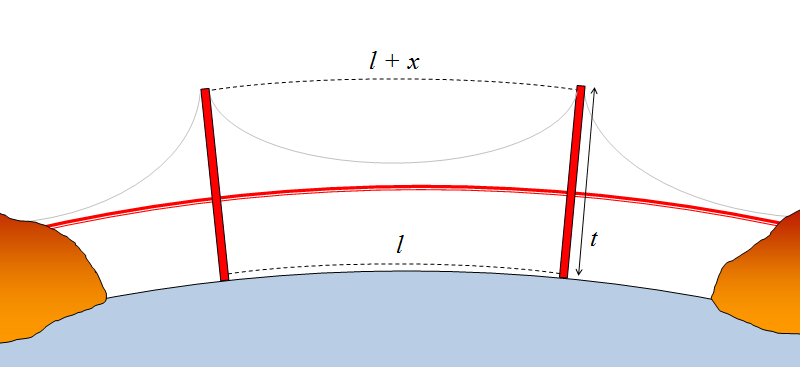
\includegraphics[width=0.95\linewidth]{bdoaa20_r_01}
\end{figure} 

The Golden Gate Bridge, possibly the most photographed bridge in the World, spans the opening of San Francisco Bay. Completed in 1937, it boasts two towers of height $230~\mathrm{m}$ and these are $1,280~\mathrm{m}$ apart. Because of the curvature of the Earth, the towers are a little wider apart at the top than at the bottom (the diagram below is exaggerated, you may not observe such curvature with your eyes!).\prr 

`দি গোল্ডেন গেট ব্রিজ'-- সম্ভবত বিশ্বের সবচেয়ে বেশিবার ছবিতে আবদ্ধ সেতু, সান ফ্রান্সিসকো বে-র প্রবেশমুখের দুইপ্রান্তকে সংযুক্ত করেছে। ১৯৩৭ সালে এর নির্মাণকাজ শেষ হয়। সেতুটির গর্ব এর দুটি টাওয়ার- যাদের উচ্চতা ২৩০ মিটার এবং এদের মধ্যবর্তী দূরত্ব ১,২৮০ মিটার। পৃথিবী পৃষ্ঠের বক্রতার কারণে, টাওয়ার দুটির ভিত্তির চেয়ে শীর্ষ দুটির দূরত্ব সামান্য বেশি (নিচের ছবিটা অতিরঞ্জিত, খালি চোখে এমন বক্রতা নাও দেখতে পারো!)



\begin{enumerate}[a.]
	\item Calculate the difference between the towers at their tops compared to the difference between bases (denoted as $x$). \m{3}
	
	ভিত্তির তুলনায় শীর্ষ দুটির দূরত্ব $x$ কত বেশি, তা নির্ণয় করো। 
	
	\item How far is your horizon standing at top of Golden Gate Bridge? (suppose your own height is negligible for this scenario) \m{3}
	
	গোল্ডেন গেট ব্রিজের একেবারে শীর্ষে দাঁড়ালে, দিগন্ত তোমার কত দূরে দেখাবে? (ধরে নাও এই দৃশ্যকল্পে তোমার উচ্চতা একেবারেই নগণ্য!) 
\end{enumerate}


\clearpage
\section{Positional Astronomy -- স্থানাংক জ্যোতির্বিজ্ঞান}


\pr{Abir's Observation}{R}{2018}

আবির জুন মাসের ২২ তারিখে আকাশ পর্যবেক্ষণ করছিল। বিকেলে কোন এক সময় সে দেখে সূর্যের কারণে তার নিজের ছায়ার দৈর্ঘ্য $0.405~\mathrm{meter}$ যেখানে তার উচ্চতা $1.5~\mathrm{meter}$।\prr

আবার সূর্যাস্তের সময় আবির লক্ষ্য করল যে সূর্যাস্তের সময় শুক্রগ্রহের উন্নতি কোণ হল  $a_\Venus=+19.36^\circ$ (মানে একেবারে মাটি থেকে বা দিগন্ত থেকে শুক্রগ্রহ $19.36$ ডিগ্রি উপরে আছে)।

\begin{enumerate}[a.]
	\item বিকেলের ঐ সময় সূর্যের উন্নতি কোণ কত ছিল? \m{2}
	
	\item সে সূর্যাস্তের কতক্ষণ পর শুক্রগ্রহকে অস্ত যেতে দেখবে? \m{2}
	
	\item আবির যে স্থান থেকে পর্যবেক্ষণ করছিল সেখানকার অক্ষাংশ কত? \m{3}
\end{enumerate}


\pr{Daylight}{R}{2018}

নিচে প্রদত্ত গ্রাফ টি $0^\circ$, $30^\circ$ N, $50^\circ$ N এবং $60^\circ$ N এই 8 টি অক্ষাংশে সারা বছরের প্রতিটা দিন কত ঘণ্টা করে দিনের আলো থাকে সেটা দেখানো হচ্ছে-

\begin{figure}[H]
	\centering
	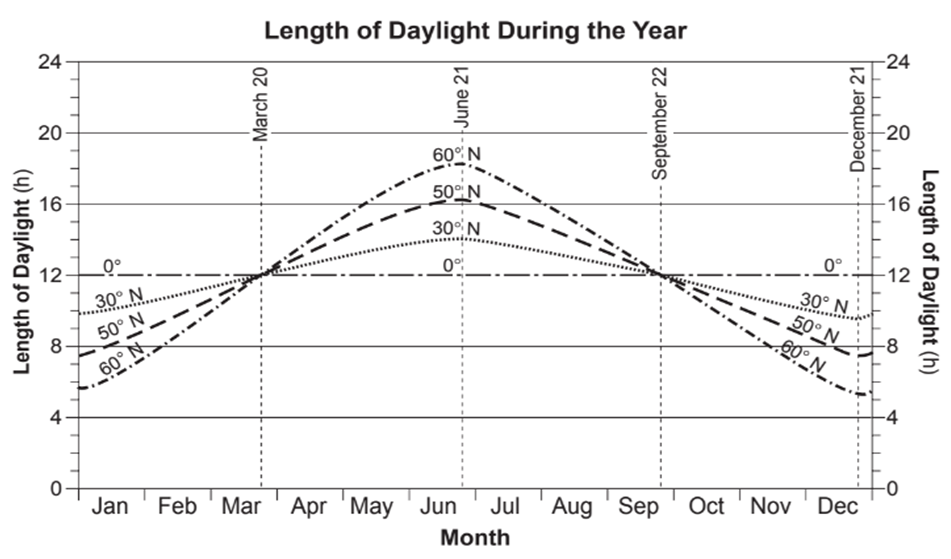
\includegraphics[width=0.9\linewidth]{bdoaa18_r_moon}
\end{figure}  

\begin{enumerate}[a.]
	\item $30^\circ$ N অক্ষাংশে ১ জানুয়ারি দিনে কতক্ষণ সূর্যের আলো পাওয়া যাবে? \m{2}
	
	\item জুনের ২১ তারিখে গ্রাফে দেখানো কোন অক্ষাংশে সূর্যোদয় আগে হবে? \m{2}
	
	\item ২০শে মার্চ এবং ২২শে সেপ্টেম্বর তারিখে কেন ৪ টি latitude এই দিনে সমান সময় সূর্যের আলো পাওয়া যাবে কেন? \m{3}
\end{enumerate}


\pr{Visibility of Bangabandhu Satellite 1}{R}{2018}

১২ মে বাংলাদেশের প্রথম ভূস্থির উপগ্রহ উৎক্ষেপিত হয়। ভূস্থির উপগ্রহ থেকে পৃথিবীকে দেখলে পৃথিবীর পৃষ্ঠের একটি নির্দিষ্ট ভাগই দেখা যায় এবং পৃথিবী থেকেও একটি নির্দিষ্ট অক্ষাংশ পর্যন্ত মানুষ উপগ্রহটিকে দেখতে পারে।

\begin{enumerate}[a.]
	\item ভূস্থির উপগ্রহ পৃথিবী থেকে কত উচ্চতায় অবস্থিত? \m{3}
	
	\item ভূস্থির উপগ্রহ থেকে একটি নির্দিষ্ট মুহূর্তে পৃথিবীর শতকরা কত অংশ দেখা যায়? \m{3}
	
	\item সর্বোচ্চ কত অক্ষাংশের মানুষ একে পর্যবেক্ষণ করতে পারবে? (ছবি এঁকে ব্যাখ্যা কর) \m{3}
	
	\item বঙ্গবন্ধু-১ স্যাটেলাইট ঠিক ইন্দোনেশিয়ার মাথার উপরে অবস্থিত। অর্থাৎ, এটি সরাসরি বাংলাদেশের উপর নয়। ইন্দোনেশিয়ার দ্রাঘিমা যদি $110^\circ$ পূর্ব হয়, তাহলে বাংলাদেশ থেকে কত ডিগ্রি কোণে সর্বোচ্চ ভালো পাওয়া যাবে? বাংলাদেশের দ্রাঘিমা $90^\circ$ পূর্ব। \m{4} 
\end{enumerate}


\pr{দিনের বেলায় আকাশে চাঁদ!}{R}{2019}


\begin{figure}[H]
	\centering
	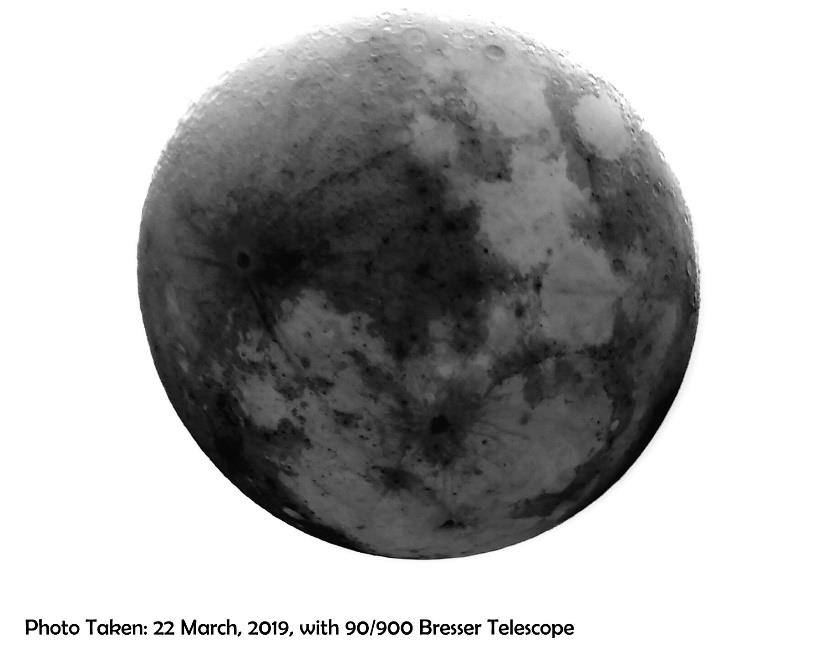
\includegraphics[width=0.9\linewidth]{bdoaa19_r_moon}
\end{figure}  
\begin{enumerate}[a.]

	\item চাঁদ থেকে পৃথিবীর দূরত্ব $d$ এবং পৃথিবীর ব্যাসার্ধ $r$ হলে চাঁদে অবস্থানকারী মহাকাশচারীর কাছে পৃথিবী পুরোপুরি উদয় হতে কতক্ষণ সময় লাগবে? \m{2}

	
	\item সাধারণত দিনের আকাশের পৃষ্ঠ ঔজ্জ্বল্য (Surface magnitude) থাকে \par $\mu_\leftmoon= 4~\mathrm{magnitude/arcsecond^2}$। যদি পূর্ণিমা চাঁদের আপাত উজ্জ্বলতা $m_\leftmoon=-12.6$ এবং কৌণিক ব্যাস $\theta_\leftmoon= 31''$ ($''=$ arcsecond) হয় তাহলে, দিনের আকাশে চাঁদ দেখা যাবে কিনা? \m{3}
	
	\item ধর একদিন বাংলাদেশ থেকে পূর্ণ সূর্যগ্রহণ দেখা গেল যখন সূর্য একদম আমাদের $(23.5^\circ~\mathrm{N})$ মাথার উপরে ছিল। চাঁদ বিষুবরেখা (equator) বরাবর আকাশে চলে। এই অবস্থায় চাঁদের ছায়ার আমাদের অক্ষাংশ বরাবর বেগ কত হতে হবে? \m{4}
\end{enumerate}


\pr{Long Night in Winterfell}{R}{2021}

Somewhere beyond the Wall, on a random summer solstice day, Jon Snow noted that the highest altitude of the Sun above the horizon was $40^\circ$.

নর্থের ``ওয়াল''-এর ওপাশে এক জায়গায় কোনো এক উত্তরায়ণের সময় জন স্নো খেয়াল করল দিগন্তের উপর সূর্যের সর্বোচ্চ উচ্চতা $40^\circ$।

\begin{enumerate}[a.]
	
	\item What is the latitude of that place? \m{1}
	
	ঐ স্থানের অক্ষাংশ (latitude) কত?
	
	\item What is the lowest altitude of the Sun on that day? \m{2}
	
	ঐ দিনে দিগন্তের উপর সূর্যের সর্বনিম্ন উচ্চতা কত?
	
	\item Suppose Jon is beyond the Wall, and $N$ days have passed since January 1. The declination of the Sun can be approximated by the following equation:
	
	মনে করো জন ``প্রাচীরের ঐপাশ''-এ অবস্থান করছে এবং ১লা জানুয়ারি হতে $N$ দিন অতিবাহিত হয়েছে। আমরা সূর্যের বিষুবলম্ব নিম্নোক্তভাবে নির্ণয় করতে পারি:
	
	\[
	\sin\delta_{\odot}
	=0.39795\cdot
	\cos\left[0.98563\cdot(N-173)\right]
	\]
	
	What will be the highest altitude of the Sun on August 1? \m{2}
	
	১লা আগস্টে সূর্যের আকাশে সর্বোচ্চ উচ্চতা কত হবে?
	
	\item Approximately, for how many days of the year will the Sun not rise at the location where Jon is making his observations? Ignore atmospheric refraction. \m{3}
	
	জন স্নো যে স্থানে থেকে তার পর্যবেক্ষণ চালাচ্ছে, সে স্থানে আনুমানিকভাবে কত দিন সূর্যোদয় হবে না? বায়ুমণ্ডলের প্রতিসরণ উপেক্ষা করো।
	
\end{enumerate}



\pr{Culmination - উদয়}{R}{2022}

\textit{N.B: Proper conditions and diagrams are necessary for solution of all the parts below.}

লক্ষণীয় এই সমস্যার সমাধানের জন্য উপযুক্ত শর্ত এবং চিত্র আঁকা আবশ্যকীয়।

\begin{enumerate}[a.]
	
	\item Calculate the height of the upper and lower culmination of the star El-Nat ($\beta$ Tau) the city of Irpin, Kyiv region ($\phi=50^\circ31'$). The declination of the star $\delta=+28^\circ37'$.
	
	বৃষরাশির তারা অত্রিকে ($\beta$ Tau) ইরপিন শহর (অক্ষাংশ $\phi=50^\circ31'$) থেকে দেখলে সর্বোচ্চ এবং সর্বনিম্ন উন্নতি কত হবে? তারাটির বিষুবলম্ব $\delta=+28^\circ37'$।
	
	\item Under what conditions will the star never rise in Genichesk ($\phi=46^\circ10'$)?
	
	কোন শর্তে তারাটিকে Genichesk শহরে ($\phi=46^\circ10'$) কখনও উদয় হতে দেখা যাবে না?
	
	\item What time is the star Aldebaran ($\alpha$ Tau, $\delta=16^\circ33'$) located above the horizon in Kiev during the starry day?
	
	কোন সময় ধরে হলদীবরণ তারাকে ($\alpha$ Tau, $\delta=16^\circ33'$) কিভ শহরের আকাশে দিগন্তের উপরে দেখা যাবে?
	
\end{enumerate}





% Problems here

\clearpage

\section{Celestial Mechanics}

% Problems here

\clearpage

\section{Stellar Astrophysics}

% Problems here

	
\end{document}